\begin{center}
\begin{tikzpicture}
    \node (src) {};

    % pair (pair _ _) _ -- _
    % pair (pair _ _) _
    \node[crossing, right=1cm of src] (0) {};
   
    %% pair _ _
    \node[crossing, above right=1cm and 0.5cm of 0] (00) {};
    \node[gate, above right=0.25cm and 0.5cm of 00] (000) {\phantom{unit}};
    \node[gate, below right=0.25cm and 0.5cm of 00] (001) {\phantom{unit}};
    \node[pair, right=1.75cm of 00] (01) {$+$};

    \draw (00) |- (000);
    \draw (00) |- (001);
    \draw (01) |- (000);
    \draw (01) |- (001);
    \node[above right=-0.1cm and -0.1cm of 000] (label000) {$M_0$};
    \node[below right=-0.1cm and -0.1cm of 001] (label001) {$M_1$};
    \node[subcircuit, fit=(00) (000) (001) (01) (label000) (label001)] (00-01) {};
    \node[above right=-0.1cm and -0.1cm of 00-01] (label00-01) {$M_2$};
    %% end pair

    %% _
    \node[gate, below right=1cm and 0.5cm of 0] (02) {\phantom{unit}};
    \node[above right=-0.1cm and -0.1cm of 02] (label02) {$M_3$};
    %% end

    \node[pair, right=3cm of 0] (1) {$+$};

    \draw (0) |- (00);
    \draw (0) |- (02);
    \draw (1) |- (01);
    \draw (1) |- (02);
    \node[subcircuit, fit=(0) (00-01) (02) (1) (label00-01) (label02)] (0-1) {};
    \node[above right=-0.1cm and -0.1cm of 0-1] (label0-1) {$M_4$};
    % end pair

    % _
    \node[gate, right=1cm of 1] (2) {\phantom{unit}};
    \node[above right=-0.1cm and -0.1cm of 2] (label2) {$M_5$};

    \draw (1) -- (2);
    % end _

    \node[right=1cm of 2] (tgt) {};

    \draw (src) -- (0);
    \draw (2) -- (tgt);
    \node[subcircuit, fit=(src) (0-1) (2) (tgt) (label0-1) (label2)] (src-tgt) {};
    \node[above right=-0.1cm and -0.1cm of src-tgt] (labelsrc-tgt) {$M_6$};
\end{tikzpicture}
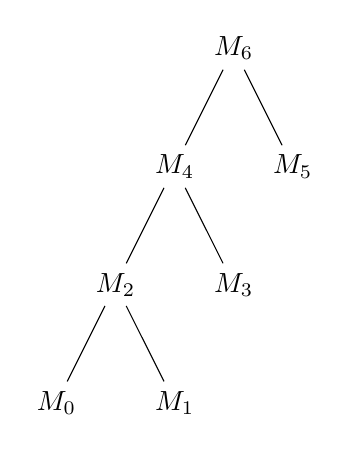
\begin{tikzpicture}
    \node {$M_6$}
        child { node {$M_4$}
            child { node {$M_2$}
                child { node {$M_0$} }
                child { node {$M_1$} }
            }
            child { node {$M_3$} }
        }
        child { node {$M_5$} };
\end{tikzpicture}
\end{center}
